\graphicspath{{images/}}

\section{Determinante}

    \begin{definition}{Determinante}
        gibt an, ob eine Matrix invertierbar ist
        \begin{equation*}
            \det(A)
            \left\{
                \begin{array}{lll}
                    \neq 0   &\Rightarrow    & A^{-1} \text{ existiert }\\
                    = 0     &\Rightarrow    & A^{-1} \text{ existiert nicht }
                \end{array}
            \right.
        \end{equation*}
    \end{definition}

    

    \begin{definition}{Geometrische Interpretation} der Determinante:\\
        \begin{minipage}{0.7\linewidth}
        Fläche im $\mathbb{R}^2$ und Volumen im $\mathbb{R}^3$\\
        durch eine Matrix A aufgespannt:
        $$A = |\vec{a} \times \vec{b}| = |\det(A)|$$
        \end{minipage}
        \begin{minipage}{0.25\linewidth}
            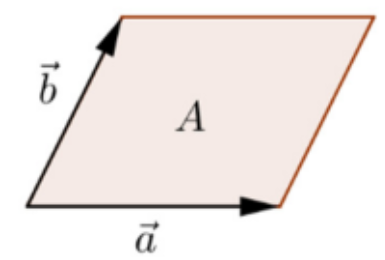
\includegraphics[width=1\linewidth]{images/determinante.png}
        \end{minipage}
    \end{definition}

   
    
    \begin{theorem}{Eigenschaften von Determinanten}{\footnotesize mit $A, B \in \mathbb{R}^{n \times n}$, $\lambda \in \mathbb{R}$}\\
        \begin{minipage}{0.5\linewidth}
            \begin{itemize}
                \item $\det(A \cdot B) = \det(A) \cdot \det(B)$
                \item $\det(\lambda \cdot A) = \lambda^n \cdot \det(A)$
                \item $\det(A) = 0 \Leftrightarrow A$ ist singulär
                
            \end{itemize}
        \end{minipage}
        \begin{minipage}{0.5\linewidth}
            \begin{itemize}
                \item $\det(E) = 1$
                \item \vspace{1mm}
                \item $\det(A^T) = \det(A)$
                \vspace{1mm}
                \item $\det(A^{-1}) = \frac{1}{\det(A)}$
            \end{itemize}
        \end{minipage}

        \vspace{1mm}

        {\footnotesize $E$ = Einheitsmatrix}
    \end{theorem}

    \begin{formula}{Determinante $1\times 1$-Matrix} $\det(A)=A_{11}$
    \end{formula}
    
    \begin{formula}{Determinante $2 \times 2$-Matrix}
        $A = \begin{psmallmatrix} a & b \\ c & d \end{psmallmatrix}$
        
        $\det(A) = |A| = a \cdot d - b \cdot c$
    \end{formula}

    \begin{minipage}{0.7\linewidth}
    \begin{formula}{Determinante $3 \times 3$-Matrix}
        $A = \begin{psmallmatrix} a & b & c \\ d & e & f \\ g & h & i \end{psmallmatrix}$

        $|A| = a \cdot e \cdot i + b \cdot f \cdot g + c \cdot d \cdot h - c \cdot e \cdot g - b \cdot d \cdot i - a \cdot f \cdot h$
    \end{formula}
    \end{minipage}
    \begin{minipage}{0.3\linewidth}
        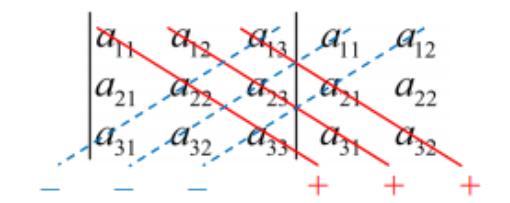
\includegraphics[width=1\linewidth]{images/determinante_3x3.png}
    \end{minipage}
    
    \begin{concept}{Determinante $n \times n$-Matrix}\\
        $\det(A) = |A| = \sum_{i=1 \text{ oder } j=1}^{n} (-1)^{i+j} \cdot a_{ij} \cdot |A_{ij}|$
        \begin{itemize}
            \item Entwicklung nach Zeile: $j$ bei $\Sigma$ und wähle eine feste Zeile $i$
            \item Entwicklung nach Spalte: $i$ bei $\Sigma$ und wähle eine feste Spalte $j$
            \item $a_{ij}$ ist das Element der Matrix $A$ in der $i$-ten Zeile und $j$-ten Spalte
            \item $|A_{ij}|$ ist die Determinante der $(n-1) \times (n-1)$-Matrix, die entsteht
        \end{itemize}

        \vspace{1mm}

        \textcolor{pink}{Tipp:} Entwickeln nach Spalte oder Zeile mit den meisten Nullen!
    \end{concept}

    \begin{KR}{Tricks und Tipps}
        \begin{itemize}
            \item hat $A$ eine Nullzeile oder -spalte, so ist $\det(A) = 0$
            \item hat $A$ zwei gleiche Zeilen oder Spalten, so ist $\det(A) = 0$
            \item $\det(A) \neq 0$ $\Rightarrow$ Spalten/Zeilen sind linear unabhängig
        \end{itemize}
    \end{KR}

    \begin{formula}{Determinante mit Gauss} Spezialfall \textcolor{pink}{Dreiecks- /Diagonalmatrix}

        Wende Gauss-Algorithmus an, um $A$ in Dreiecksform zu bringen.\\ Es gilt für jede Dreiecksmatrix oder Diagonalmatrix $D$:
        $$\det(D) = (-1)^k \prod_{i=1}^n d_{ii}$$
        {\small $k$ = Anzahl der Zeilen-Vertauschungen}
        
        \vspace{1mm}

        Bei Zeilen-Vertauschungen ändert sich das Vorzeichen von $\det(A)$\\ 
        $\det(A)$ verändert sich nicht bei Zeilen-Additionen/-Multiplikationen

        \vspace{1mm}

        {\small Bei Skalarmultiplikationen ändert sich $\det(A)$ um den Skalierungsfaktor (am besten einfach keine Skalarmultiplikationen durchführen)}
    \end{formula}




